В результате пьезоэлектрического эффекта происходит деформация
кристаллической решетки и данный эффект будет влиять на
КДО, а именно, будет меняться  угловое положение и профиль кривой.
Изменение профиля КДО может быть вызвано исходя из следующих
соображений:

1. Изменение профиля происходит за счет изменения структурного фактора, но
данный эффект не рассматривается в данной работе. На первом этапе ограничимся
случаем однородной деформации решетки кристалла. Такая деформация описывается
 матрицей пьезомодулей, вследствие чего относительное расположение атомов
 внутри элементарной ячейки остается постоянным, как и структурный фактор.

 \begin{figure}[H]
   \centering
   
\includegraphics[width=0.3\textwidth]{images/none.png}
   \caption{Изменение профиля собственной КДО кристалла LGT под воздействие электрического поля}
   \label{ris:self_kdo_deformation}
 \end{figure}


2. Профиль кривой также может изменяться изменения дисперсионности схемы.
При пьезоэффекте меняется межплоскостное расстояние, а значит и угол Брэгга, таким
образом может возникать дисперсионное уширение КДО и изменение интегральной интесивности
отраженного пучка (см. \ref{sec:dispersion_cal_an_exp}). Для оценки уширения был
проведен расчет, который заключался в оценки полуширины результирующей двухкристальной КДО
в зависимости от изменения угла Брэгга образца (рис. \ref{ris:FWHM_diference_bragg})
%(отлажить по оси х дельта брэгга)
\begin{figure}[H]
  \centering
  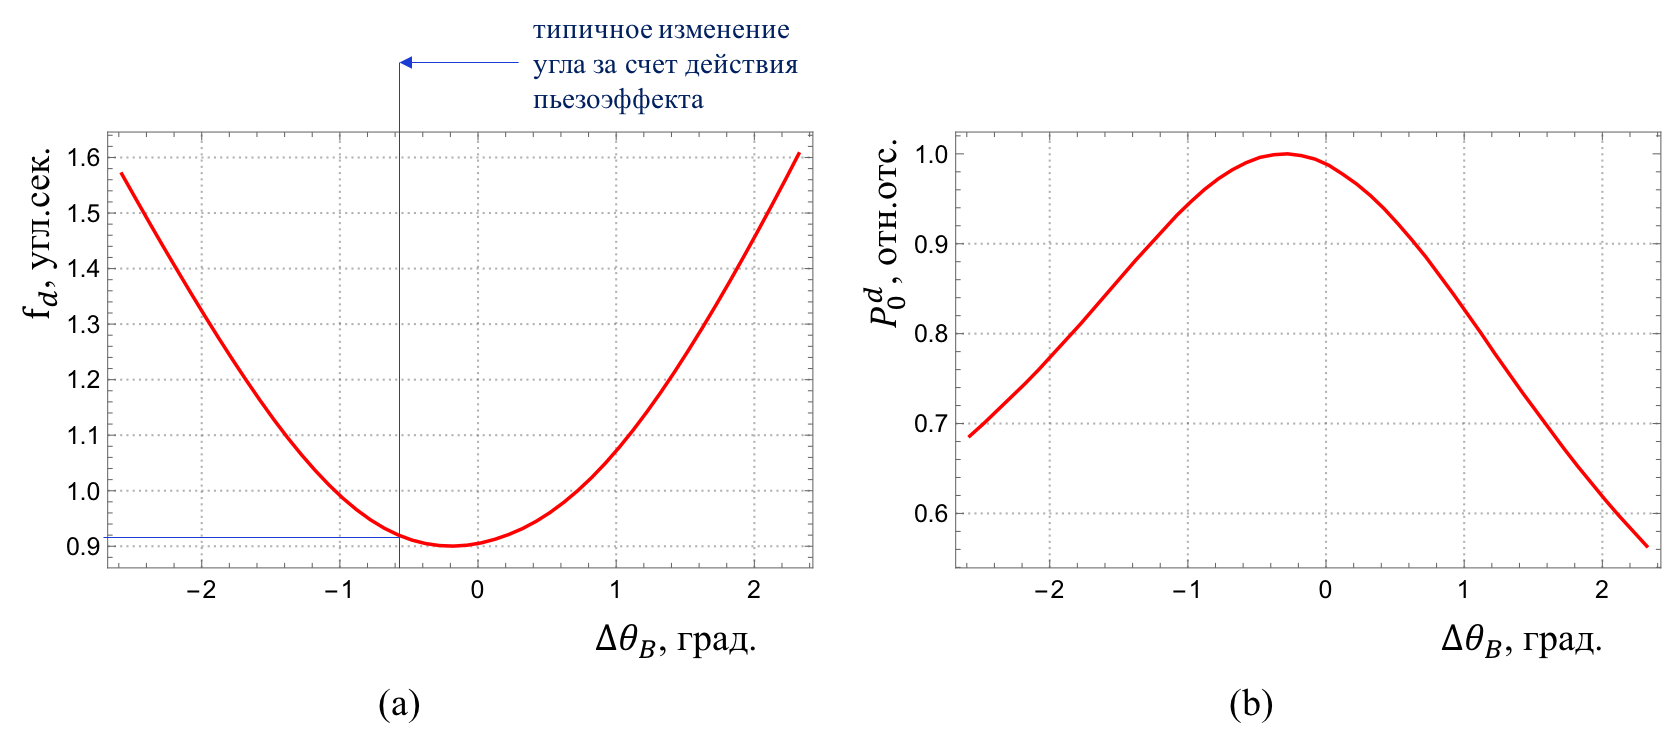
\includegraphics[width=0.95\textwidth]{images/delta_bragg_dispers.png}
  \caption{Зависимость (a) полуширины двухкристальной КДО $f_d$ и (b) амплитуды в максимуме КДО  $P^d_0$
   от разности углов Брэгга $\Delta\theta_B =\theta_B^S-\theta_B^M $ кристаллов
  образца (M) и монохроматора (S). Отсчет ведется от угла Брэгга моноохроматора $\theta_B^M = 21.6785 ^o$ - Si (440),
  в качестве образца был взят кристалл LGT с плоскостью отражения (246) $\theta_B^S = 21.0328 ^o$}
  \label{ris:FWHM_diference_bragg}
\end{figure}

Из результатов можно сделать вывод, как и следовало ожидать минимальная полуширина соответсвует
случаю когда углы Брэгга обоих кристаллов в точности совпадают. С увеличением
дисперсионности изменение полуширины выходит на линейную зависимость, т.е.
имеет монотонный характер. При характерных для пьезоэффекта сдвигах КДО (до 10 угл.сек.)
изменение полуширины за счет изменения дисперсионности схемы составляет
величину меньшую разрешающей способности дифрактометра, т.е полуширина и
амплитуда остается постоянной
 (рис. \ref{ris:FWHM_diference_bragg_KDO}).

\begin{figure}[H]
  \centering
  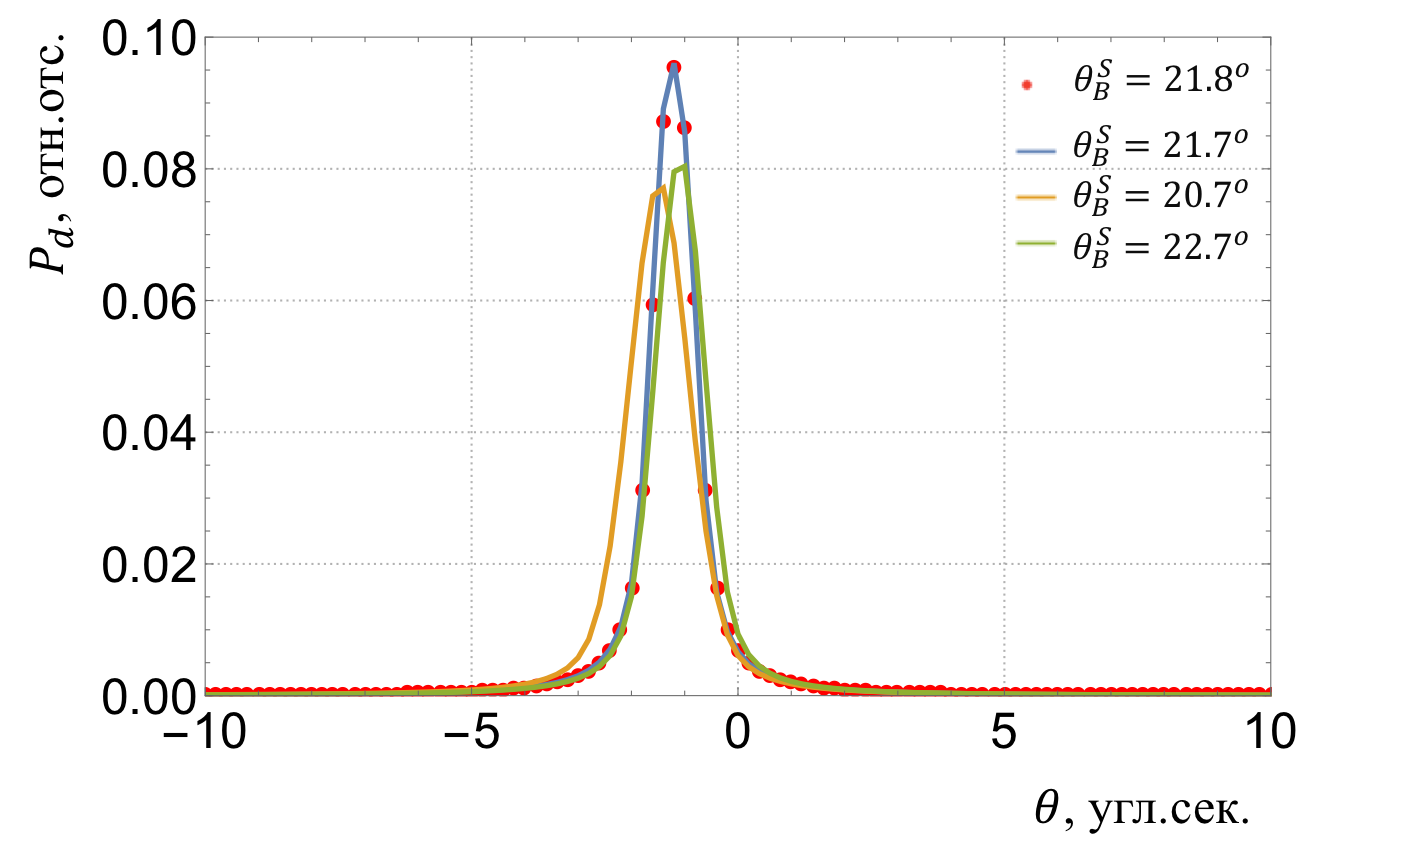
\includegraphics[width=0.8\textwidth]{images/FWHM_diference_bragg_KDO.png}
  \caption{КДО для разныой степени дисперсионности схемы, $\theta_B^M = 21.6785 ^o$}
  \label{ris:FWHM_diference_bragg_KDO}
\end{figure}

Для того, чтобы добиться существенного изменения изменения кривой нужно
иметь угловую отстройку порядка градуса, такое изменение угла Брэгга
соответсвует изменению межплоскостного расстояния на величину $d/d_0 \simeq 0.03$
процентов, а такие деформации в кристалле не допустимы (при $d/d_0 > 10^{-4}$ происходит разрушение).
Таким образом в результате пьезоэффекта профиль кривой, для рассмотренных нами случаев,
должен оставаться постоянным.

Необходимо отметить, что деформации профиля КДО может происходить вследствие наличия
заряженных дефектов в кристалле, которые подвержены влиянию электрического поля. Но данный механизм
также не рассматривается в данной работе.

Данное заключение позволяется применять рассмотренные методы расчета для определения пьезоэлектрических констант,
а так же использовать времяразрешающий метод исследования (см. \ref{sec:slope_diff_piezo}).
